\chapter{Networking and the Internet}

A network is a way of 

\section{OSI Model and the TCP/IP Stack}
The Internet is an \textit{extremely} complicated system. There are many pieces that must work together in order for you to receive your cat video. Given the enormous complexity of all the interconnecting parts you would think that it might be a nightmare to understand. Luckily we can break it down into layers. 

In the late 1970s, the International Organisation for Standardisation (ISO) proposed that computer networks be organised around a seven layer model. Figure \ref{fig:OSIModel}

\begin{figure}[h!]
	\centering
	\subfloat[OSI]{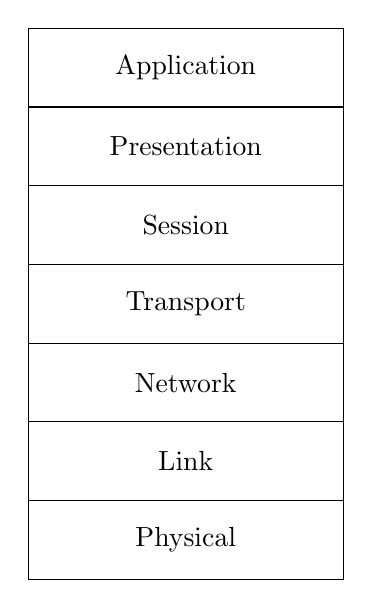
\begin{tikzpicture}
		\draw  (0,6) rectangle (4,7) node[pos=.5] {Application};
		\draw  (0,5) rectangle (4,6) node[pos=.5] {Presentation};
		\draw  (0,4) rectangle (4,5) node[pos=.5] {Session};
		\draw  (0,3) rectangle (4,4) node[pos=.5] {Transport};
		\draw  (0,2) rectangle (4,3) node[pos=.5] {Network};
		\draw  (0,1) rectangle (4,2) node[pos=.5] {Link};
		\draw  (0,0) rectangle (4,1) node[pos=.5] {Physical};
		
		\end{tikzpicture}}
	\qquad\qquad
	\subfloat[TCP/IP Stack]{\label{fig:OSIModel} 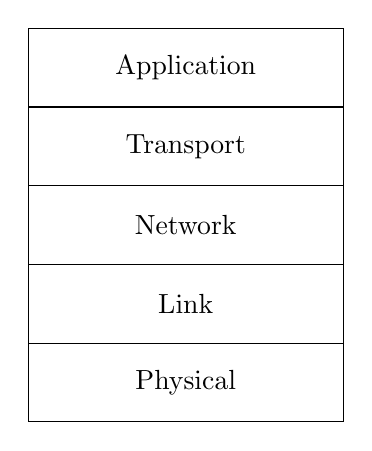
\begin{tikzpicture}
		\draw  (0,4) rectangle (4,5) node[pos=.5] {Application};
		\draw  (0,3) rectangle (4,4) node[pos=.5] {Transport};
		\draw  (0,2) rectangle (4,3) node[pos=.5] {Network};
		\draw  (0,1) rectangle (4,2) node[pos=.5] {Link};
		\draw  (0,0) rectangle (4,1) node[pos=.5] {Physical};
		
		\end{tikzpicture}}
	\caption{\label{fig:FlynnsTaxo} The two different layering models for }
\end{figure}

